\documentclass[cn,hazy,green,12pt,normal]{elegantnote}

\title{作业3解答}
\author{24Spring 回归分析}
\date{\today}

\usepackage{array}

\usepackage{amsmath, amssymb, bm, color, framed, graphicx, hyperref, mathrsfs, fontspec, geometry, extarrows, amsthm}

\DeclareMathOperator{\e}{\!\!\;\mathrm e}
\DeclareMathOperator{\Cov}{Cov}
\DeclareMathOperator{\Var}{Var}
\DeclareMathOperator{\var}{var}
\DeclareMathOperator{\tr}{tr}
\DeclareMathOperator{\diag}{diag}
\newcommand{\p}{\partial}
\renewcommand{\d}{\mathop{}\!\mathrm{d}}
\newcommand{\MR}{\mathbb R}
\newcommand{\MC}{\mathbb C}
\newcommand{\MF}{\mathbb F}
\newcommand{\MZ}{\mathbb Z}
\newcommand{\MN}{\mathbb N}
\newcommand{\MCF}{\mathscr F}
\renewcommand{\Re}{\operatorname{Re}}
\renewcommand{\Im}{\operatorname{Im}}
\renewcommand{\boldsymbol}{\bm}
\renewcommand{\i}{\mathrm i}

\DeclareMathOperator{\Arg}{Arg}
\DeclareMathOperator{\I}{I}
\usepackage{tkz-euclide}
\numberwithin{equation}{section}
\numberwithin{subsection}{section}

\lstset{
    language=R,
    basicstyle=\ttfamily,
    keywordstyle=\color{blue},
    commentstyle=\color{gray},
    frame=single,
    breaklines=true
}

\begin{document}
\maketitle
\begin{homework}
\end{homework}
    \begin{figure}[!htbp]
        \centering
        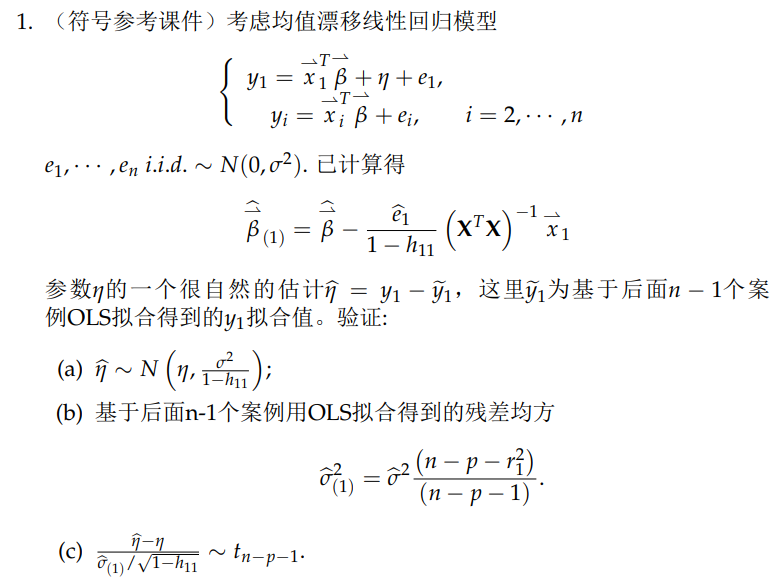
\includegraphics[width=30em]{image/hw3_plt1.png}
    \end{figure}

\begin{proof}
 (a)      
\begin{align*}
    \hat{\eta} = y_1-x_1^T(\hat{\beta}-\dfrac{\hat{e_1}}{1-h_{11}}(X^TX)^{-1}x_1)&=(y_1-x_1^T\hat{\beta})+\dfrac{\hat{e_1}}{1-h_{11}}(x_1^T(X^TX)^{-1}x_1)\\
    &=\hat{e_1}+\dfrac{\hat{e_1}h_{11}}{1-h_{11}}\\
    &=\dfrac{\hat{e_1}}{1-h_{11}}
\end{align*}
设$d_1$表示第一个分量为1,其余分量为0的n维向量,注意到
\[\hat{e}=y-\hat{y}=(I_n-H)y=(I_n-H)(X\beta+d_1\eta+e)=(I_n-H)(d_1\eta+e)\] \[\hat{e_1}=d_1^T\hat{e}=(1-h_{11})\eta+d_1^T(I_n-H)e\sim N((1-h_{11})\eta,(1-h_{11})\sigma^2)\]
故
\[\hat{\eta}=\dfrac{\hat{e_1}}{1-h_{11}} \sim N(\eta,\dfrac{\sigma^2}{1-h_{11}})\]

\noindent (b)首先计算$RSS_{(1)}$:
\begin{align*}
    RSS_{(1)}=||(I_{n-1}-P_{X_{(1)}})y_{(1)}||^2&=y_{(1)}^Ty_{(1)}-y_{(1)}^TX_{(1)}\hat{\beta}_{(1)}\\
    &=(y^Ty-y_1^2)-(y^TX-y_1x_1^T)(\hat{\beta}-\dfrac{\hat{e_1}}{1-h_{11}}(X^TX)^{-1}x_1)\\
    &=y^Ty-y_1^2-y^TX\hat{\beta}+y_1x_1^T\hat{\beta}+y^TX\dfrac{\hat{e_1}}{1-h_{11}}(X^TX)^{-1}x_1\\
    &\quad-y_1x_1^T\dfrac{\hat{e_1}}{1-h_{11}}(X^TX)^{-1}x_1\\
    &=(y^Ty-y^TX\hat{\beta})+(-y_1^2-y_1\dfrac{\hat{e_1}h_{11}}{1-h_{11}})\\
    &\quad +(y_1x_1^T\hat{\beta}+\dfrac{\hat{e_1}}{1-h_{11}}\hat{\beta}^Tx_1)
\end{align*}
最后式子中
\[y^Ty-y^TX\hat{\beta}=RSS,\qquad -y_1^2-y_1\dfrac{\hat{e_1}h_{11}}{1-h_{11}}=-y_1(y_1+\dfrac{\hat{e_1}h_{11}}{1-h_{11}}),\]
\[ y_1x_1^T\hat{\beta}+\dfrac{\hat{e_1}}{1-h_{11}}\hat{\beta}^Tx_1=y_1\hat{y_1}+\dfrac{\hat{e_1}}{1-h_{11}}\hat{y_1}=\hat{y_1}(y_1+\dfrac{\hat{e_1}}{1-h_{11}})\]
因此
\begin{align*}
    LHS&=RSS+y_1(\hat{y_1}-y_1)+\dfrac{\hat{e_1}}{1-h_{11}}\hat{y_1}-\dfrac{\hat{e_1}h_{11}}{1-h_{11}}y_1\\
    &=RSS+y_1(-\hat{e_1}-\dfrac{\hat{e_1}h_{11}}{1-h_{11}})+\dfrac{\hat{e_1}}{1-h_{11}}\hat{y_1}\\
    &=RSS-\dfrac{\hat{e_1}^2}{1-h_{11}}
\end{align*}
从而\[\hat{\sigma^2}_{(1)}=\dfrac{RSS_{(1)}}{n-p-1}=\dfrac{(n-p)\hat{\sigma^2}-r_1^2\hat{\sigma^2}}{n-p-1}=\dfrac{n-p-r_1^2}{n-p-1}\hat{\sigma^2}\]

\noindent (c)根据(a)的结论$\hat{\eta} \sim N(\eta,\dfrac{\sigma^2}{1-h_{11}})$,可得
$$
\dfrac{\hat{\eta}-\eta}{\sqrt{\frac{\sigma^2}{1-h_{11}}}}\sim N(0,1).
$$
注意到$\hat{\sigma}^2_{(1)}$是对剩下n-1个样本回归后的残差均方,因此
$$
\dfrac{(n-p-1)\hat{\sigma}^2_{(1)}}{\sigma^2} \sim \chi_{n-p-1}^2.
$$
接下来需要证明$\hat{\eta}$与$\hat{\sigma}^2_{(1)}$独立。根据(b)的结论,$(n-p-1)\hat{\sigma}^2_{(1)} = RSS_{(1)} = RSS - \dfrac{\hat{e_1}^2}{1-h_{11}}$,其中
\begin{align*}
    RSS &= y^T (I_n-H) y, \\
    &= (X\beta+d_1\eta+e)^T (I_n-H) (X\beta+d_1\eta+e), \\
    &= (d_1\eta+e)^T (I_n-H) (d_1\eta+e), \\
    &= (1-h_{11}) \eta^2 + 2 \eta d_1^T (I_n-H) e + e^T (I_n-H) e. \\
    \dfrac{\hat{e_1}^2}{1-h_{11}} &= \dfrac{\left[(1-h_{11})\eta + d_1^T (I_n-H) e\right]^2}{1-h_{11}}, \\
    &= (1-h_{11}) \eta^2 + 2 \eta d_1^T (I_n-H) e + e^T \dfrac{(I_n-H)d_1d_1^T(I_n-H)}{1-h_{11}} e.
\end{align*}
于是
$$
RSS_{(1)}=e^T(I_n-H-\dfrac{(I_n-H)d_1d_1^T(I_n-H)}{1-h_{11}})e.
$$
由(a)的计算过程可得$(1-h_{11}) (\hat{\eta}-\eta) = d_1^T (I_n-H) e$,注意到
\begin{align*}
    & \left[I_n-H-\dfrac{(I_n-H)d_1d_1^T(I_n-H)}{1-h_{11}}\right](I_n-H)d_1 \\
    =& (I_n-H)d_1-\dfrac{(I_n-H)d_1[d_1^T(I_n-H)d_1]}{1-h_{11}} \\
    =& (I_n-H)d_1-(I_n-H)d_1 \\
    =& 0,
\end{align*}
由PPT上相关定理可得$(1-h_{11}) (\hat{\eta}-\eta)$与$RSS_{(1)}$独立,则$\hat{\eta}$与$\hat{\sigma}^2_{(1)}$独立。再利用t分布的定义,即得
\[\dfrac{\dfrac{\hat{\eta}-\eta}{\sqrt{\frac{\sigma^2}{1-h_{11}}}}}{\dfrac{\hat{\sigma}_{(1)}}{\sigma}}=\dfrac{\hat{\eta}-\eta}{\sigma_{(1)}/\sqrt{1-h_{11}}}\sim t_{n-p-1} \]

\end{proof}

\begin{note}
   (1) 参考文献定理4.4.1\cite{王松桂1999线性统计模型}:$\hat{\beta}_{(1)},\hat{\eta}$为以下模型的最小二乘估计:
    \begin{equation}\label{model 1}
            \bm y = X\bm \beta + \bm d_1 \eta + e=\begin{bmatrix}
        X&d_1
    \end{bmatrix}\begin{bmatrix}
        \bm \beta \\
        \eta\\
    \end{bmatrix}+e \quad e\sim N(0,\sigma^2I_n) 
    \end{equation}


    则此模型下的残差平方和为
    \[||y-X\hat{\bm \beta}_{(1)} + \bm d_1 \hat{\eta}||^2=y^T(I_n-P_{X,d_1})y=y^T(I_n-P_{X}-P_{d_1^{\perp}})y\]
    其中$d_1^{\perp} = (I_n-P_X)d_1,\quad P_{d_1^{\perp}}=d_1^{\perp}(d_1^{\perp T}d_1^{\perp})^{-1}d_1^{\perp T}=\dfrac{(I_n-P_X)d_1d_1^T(I_n-P_X)}{1-h_{11}}$
    
    残差平方和化简为
    \[y^T(I_n-P_{X}-P_{d_1^{\perp}})y=y^T(I_n-P_{X})y^T-y^TP_{d_1^{\perp}}y=RSS-\dfrac{\hat{e_1}^2}{1-h_{11}}\]
    正为$RSS_{(1)}$,因此由该模型\eqref{model 1}下(满足GM假设,误差服从正态)最小二乘回归系数和残差平方和的独立性,$(\hat{\beta}_{(1)},\hat{\eta})$与$RSS_{(1)}$独立。

    (2)独立性也可以通过以下方式说明:由正态假设得$\hat{\beta}_{(1)}$与$RSS_{(1)}$独立,$y_1$只依赖于$e_1,\quad RSS_{(1)}$只依赖于$e_2,\dots,e_n$,因此$y_1$与$RSS_{(1)}$独立。进而$\hat{\eta}=y_1-x_1^T\hat{\beta}_{(1)}$与$RSS_{(1)}$独立。

    (3) 由(1),$\hat{\beta}_{(1)},\hat{\eta}$为均值漂移模型$\beta,\eta$的无偏估计。注意这时$\hat{\beta}=(X^TX)^{-1}X^T\bm y = (X^TX)^{-1}X^T(X\bm \beta + \bm d_1 \eta + e)$不是$\beta$无偏估计。

\end{note}
\newpage

\begin{homework}
\end{homework}
    \begin{figure}[!htbp]
        \centering
        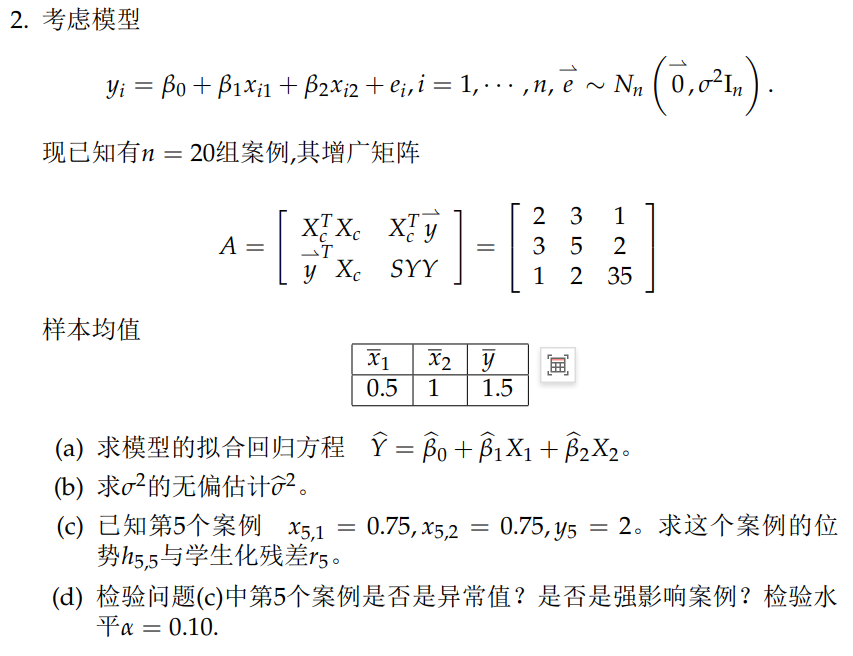
\includegraphics[width=30em]{image/hw3_plt2.png}
    \end{figure}

\begin{proof}[\solutionname]
(a) \[\begin{bmatrix}
    \hat{\beta_1}\\
    \hat{\beta_2}\\
\end{bmatrix}=(X_c^TX_c)^{-1}X_c^Ty=\begin{bmatrix}
    2&3\\
    3&5\\
\end{bmatrix}^{-1}\begin{bmatrix}
    1\\
    2\\
\end{bmatrix}=\begin{bmatrix}
    -1\\
    1\\
\end{bmatrix},\quad \hat{\beta_0}=\Bar{y}-(\Bar{x_1},\Bar{x_2})\begin{bmatrix}
    \hat{\beta_1}\\
    \hat{\beta_2}\\
\end{bmatrix}=1\]
回归方程
\[\hat{Y}=1-X_1+X_2\]
\noindent (b) \[RSS=SYY-(y^TX_c)(X_c^TX_c)^{-1}(X_c^Ty)=35-(1,2)\begin{bmatrix}
    2&3\\
    3&5\\
\end{bmatrix}^{-1}\begin{bmatrix}
    1\\
    2\\
\end{bmatrix}=34,\quad \hat{\sigma}^2=RSS/(n-3)=2\]
\end{proof}

\noindent (c) \[h_{55}=\frac{1}{n}+(x_5-\Bar{x})^T(X_c^TX_c)^{-1}(x_5-\Bar{x})=\dfrac{1}{20}+(0.25,-0.25)\begin{bmatrix}
    2&3\\
    3&5\\
\end{bmatrix}^{-1}\begin{bmatrix}
    0.25\\
    -0.25\\
\end{bmatrix}=0.8625\]
\[\hat{y_5}=1-0.75+0.75=1,\quad r_5=\dfrac{\hat{e_5}}{\hat{\sigma}\sqrt{1-h_{55}}}=\dfrac{2-1}{\sqrt{2\times 0.1375}}=1.9069\]

\noindent (d)\[t_5 = |r_5|\dfrac{\sqrt{n-p-1}}{\sqrt{n-p-r_5^2}}=2.0865\ge 1.7459=t_{16}(0.05)\]为异常值。
\[D_5=\dfrac{1}{p}\dfrac{h_{55}}{1-h_{55}}r_5^2=7.6031\ge 2.44 = F_{3,17}(0.10)\]
为高影响点。
\newpage

\begin{homework}
\end{homework}
    \begin{figure}[!htbp]
        \centering
        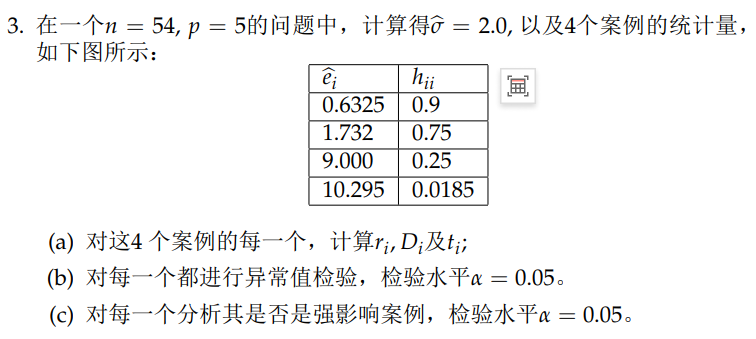
\includegraphics[width=30em]{image/hw3_plt3.png}
    \end{figure}

\begin{proof}[\solutionname]
    
\end{proof}
    \begin{figure}[!htbp]
        \centering
        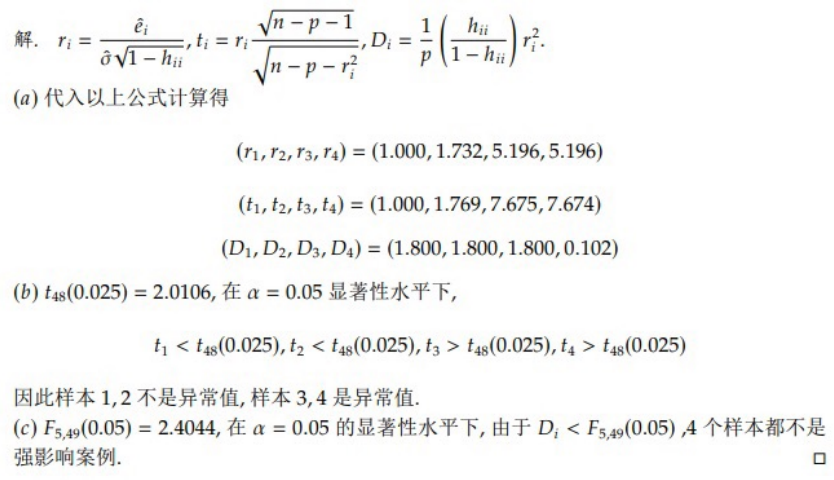
\includegraphics[width=40em]{image/hw3_plt5.png}
    \end{figure}
\begin{note}
背一下这几个公式。    
\end{note}
\newpage

\begin{homework}
\end{homework}
    \begin{figure}[!htbp]
        \centering
        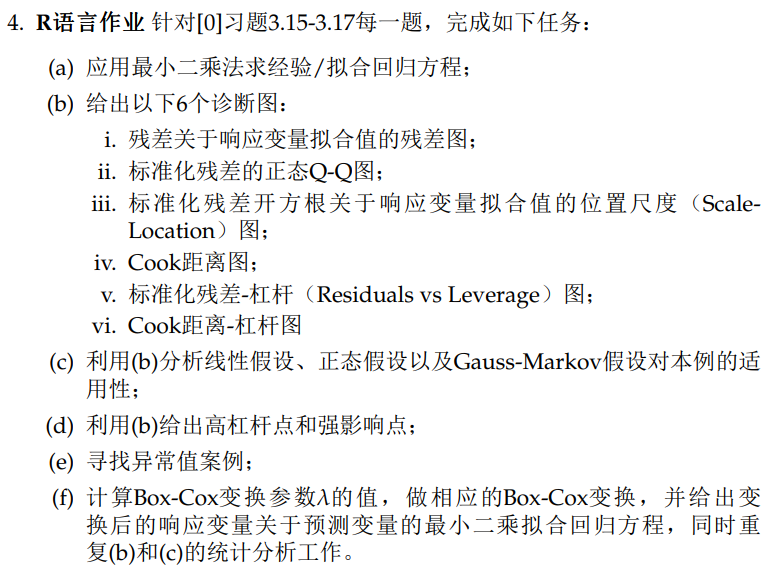
\includegraphics[width=40em]{image/hw3_plt4.png}
    \end{figure}

\begin{proof}
    见群文件hw3.rmd
\end{proof}
\begin{note}
    (1)依据第一个图判断线性假设,QQ图判断正态假设,Scale-Location 图判断等方差性。剩下几个图判断高杠杆和高影响。
    
    (2)由于$\sum_{i=1}^n h_{ii}=\tr(H)=p$,平均来看每个杠杆约为$\dfrac{p}{n}$,在实际处理时可认为$h_{ii}>\dfrac{2p}{n}$或$h_{ii}> \dfrac{3p}{n}$为高杠杆。

    (3)数据分析中$|r_i|>2$可认为异常值,不过使用outlierTest时,会综合样本量n调整p值,因此一些样例其实并不显著。考试时使用$t_{n-p-1}$检验来判断异常值。
    
    (4)数据分析中$D_i>\dfrac{4}{n-p-1}$的样本可认为高影响,也有用大于0.5或1来判断的。不过我们考试中还是使用$F_{p,n-p}$检验。

    (5)实际数据分析时,boxcox 变换可以直接采用\lstinline{lm(y^lambda~x, data = <your_data>)},不用按照\lstinline{lm((y^lambda-1)/lambda~x, data = <your_data>)}。
\end{note}

\newpage

\end{document}